% !TEX program = pdflatex
% !TEX options = --shell-escape -synctex=1 -interaction=nonstopmode -file-line-error "%DOC%"
\documentclass[notitlepage]{article}
\usepackage{float}
\usepackage{verbatim}
\usepackage{amsmath}
\usepackage{listings}
\usepackage{bm}
\usepackage{graphicx}
\usepackage{booktabs}
\usepackage{color,xcolor}
\usepackage{enumerate}
\usepackage{minted}
\usepackage{caption}
\usepackage{subcaption}

\title{Poisson-FBMP Note}
\date{}

\definecolor{dkgreen}{rgb}{0,0.6,0}
\definecolor{gray}{rgb}{0.5,0.5,0.5}
\definecolor{mauve}{rgb}{0.58,0,0.82}
\lstset{
    language=python,
    basicstyle=\footnotesize,
    numbers=left,
    numberstyle=\tiny\color{gray},
    stepnumber=2,
    numbersep=5pt,
    backgroundcolor=\color{white},
    showspaces=false,
    showstringspaces=false,
    showtabs=false,
    frame=single,
    rulecolor=\color{black},
    tabsize=2,
    captionpos=b,
    breaklines=true,
    breakatwhitespace=false,
    title=\lstname,
    keywordstyle=\color{blue},
    commentstyle=\color{dkgreen},
    stringstyle=\color{mauve},
    escapeinside={\%*}{*)},
    morekeywords={*,...}
}

\begin{document}
\newcommand{\ud}{\mathrm{d}}

\maketitle

\section{P-FBMP only fitting}

\begin{lstlisting}
def optit0mu(t0, mu, n, xmmse_star, psy_star, c_star, la):
    ys = np.log(psy_star) - np.log(poisson.pmf(c_star, la)).sum(axis=1)
    ys = np.exp(ys - ys.max()) / np.sum(np.exp(ys - ys.max()))
    t0list = np.arange(t0 - 3 * Sigma, t0 + 3 * Sigma + 1e-6, 0.2)
    mulist = np.arange(max(1e-8, mu - 3 * np.sqrt(mu)), mu + 3 * np.sqrt(mu), 0.1)
    b_mu = [max(1e-8, mu - 5 * np.sqrt(mu)), mu + 5 * np.sqrt(mu)]
    tlist_pan = np.sort(np.unique(np.concatenate([np.unique(np.hstack(np.arange(1, window-1)[:, None] + np.arange(0, 1, 1 / n))), tlist])))
    As = np.zeros((len(xmmse_star), len(tlist_pan)))
    As[:, np.isin(tlist_pan, tlist)] = c_star
    tlist_edge = np.concatenate([[tlist_pan[0] - np.diff(tlist_pan)[0] / 2], (tlist_pan[1:] + tlist_pan[:-1]) / 2, [tlist_pan[-1] + np.diff(tlist_pan)[-1] / 2]])
    diff = np.diff(tlist_edge)
    assert As.sum() == c_star.sum()
    assert sum(np.sum(As, axis=0) > 0) > 0

    def likelihood(x):
        a = x[0] * wff.convolve_exp_norm(tlist_pan - x[1], Tau, Sigma) * diff + 1e-8 # use tlist_pan not tlist
        li = -special.logsumexp(np.log(poisson.pmf(As, a)).sum(axis=1), b=ys)
        return li

    likemu = np.array([likelihood([mulist[j], t0]) for j in range(len(mulist))])
    liket0 = np.array([likelihood([mu, t0list[j]]) for j in range(len(t0list))])
    mu, t0 = opti.fmin_l_bfgs_b(likelihood, x0=[mulist[likemu.argmin()], t0list[liket0.argmin()]], approx_grad=True, bounds=[b_mu, b_t0], maxfun=50000)[0]
    return mu, t0

truth = pelist[pelist['TriggerNo'] == ent[i]['TriggerNo']]

tlist = truth['HitPosInWindow'][truth['HitPosInWindow'] < right_wave - 1]
if len(tlist) == 1:
    tlist_edge = np.array([tlist[0] - 0.5, tlist[0] + 0.5])
else:
    tlist_edge = np.concatenate([[tlist[0] - np.diff(tlist)[0] / 2], (tlist[1:] + tlist[:-1]) / 2, [tlist[-1] + np.diff(tlist)[-1] / 2]])
t_auto = (np.arange(left_wave, right_wave) / wff.nshannon)[:, None] - tlist
A = p[2] * np.exp(-1 / 2 * (np.log((t_auto + np.abs(t_auto)) / p[0] / 2) / p[1]) ** 2)

t0_t = t0_truth[i]['T0']
mu_t = len(truth)
la = mu_t * np.array([integrate.quad(lambda t : wff.convolve_exp_norm(t - t0_t, Tau, Sigma), tlist_edge[i], tlist_edge[i+1])[0] for i in range(len(tlist))]) + 1e-8

c_star_truth = np.ones_like(tlist)
wav_ans = np.sum([np.where(pp > truth['HitPosInWindow'][j], wff.spe(pp - truth['HitPosInWindow'][j], tau=p[0], sigma=p[1], A=p[2]) * truth['Charge'][j] / gmu, 0) for j in range(len(truth))], axis=0)

mu, t0 = optit0mu(t0_t, mu_t, n, np.empty(len(la))[None, :], np.array([1]), c_star_truth[None, :], la)
\end{lstlisting}

Motivation: to validate fitting process

Progress: Use true \texttt{HitPosInWindow} as \texttt{tlist}, true \texttt{T0} as \texttt{t0\_t}, length of \texttt{HitPosInWindow} as \texttt{mu\_t}. Without FBMP RGS, directly \textbf{fit} $\mu$ and $t_0$. 

Result: fitting process is not related to bias of $\mu$. 

\begin{figure}[H]
    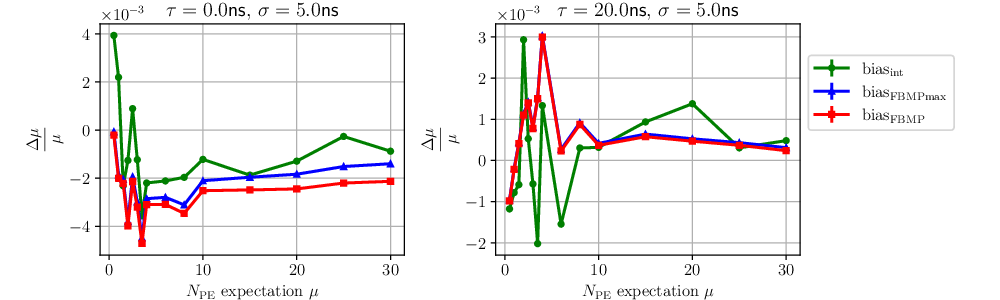
\includegraphics[width=\textwidth]{vs-biasmu-trufit.png}
\end{figure}

\section{P-FBMP with truth prior}

\begin{lstlisting}
tlist = truth['HitPosInWindow'][truth['HitPosInWindow'] < right_wave - 1]
if len(tlist) == 1:
    tlist_edge = np.array([tlist[0] - 0.5, tlist[0] + 0.5])
else:
    tlist_edge = np.concatenate([[tlist[0] - np.diff(tlist)[0] / 2], (tlist[1:] + tlist[:-1]) / 2, [tlist[-1] + np.diff(tlist)[-1] / 2]])
t_auto = (np.arange(left_wave, right_wave) / wff.nshannon)[:, None] - tlist
A = p[2] * np.exp(-1 / 2 * (np.log((t_auto + np.abs(t_auto)) / p[0] / 2) / p[1]) ** 2)
t0_t = t0_truth[i]['T0']
mu_t = len(truth)
factor = np.sqrt(np.diag(np.matmul(A.T, A)))
A = np.matmul(A, np.diag(1. / np.sqrt(np.diag(np.matmul(A.T, A)))))
la = mu_t * np.array([integrate.quad(lambda t : wff.convolve_exp_norm(t - t0_t, Tau, Sigma), tlist_edge[i], tlist_edge[i+1])[0] for i in range(len(tlist))]) + 1e-8
xmmse, xmmse_star, psy_star, nu_star, nu_star_bk, T_star, d_tot_i, d_max_i, num_i = wff.fbmpr_fxn_reduced(wave_r, A, la, spe_pre[cid]['std'] ** 2, (gsigma * factor / gmu) ** 2, factor, len(la), stop=5, truth=truth, i=i, left=left_wave, right=right_wave, tlist=tlist, gmu=gmu, para=p)
c_star = np.zeros_like(xmmse_star).astype(int)
for k in range(len(T_star)):
    t, c = np.unique(T_star[k][xmmse_star[k][T_star[k]] > 0], return_counts=True)
    c_star[k, t] = c
mu = np.average(c_star.sum(axis=1), weights=psy_star)
t0 = t0_t
\end{lstlisting}

Motivation: to prove prior used in FBMP is not the origin of $\mu$ bias. 

Progress: Use true \texttt{HitPosInWindow} as \texttt{tlist}, true \texttt{T0} as \texttt{t0\_t}, length of \texttt{HitPosInWindow} as \texttt{mu\_t}. \texttt{la} is vector of integral in each time bins. 

Result: prior used in FBMP is not the origin of $\mu$ bias. 

\begin{figure}[H]
    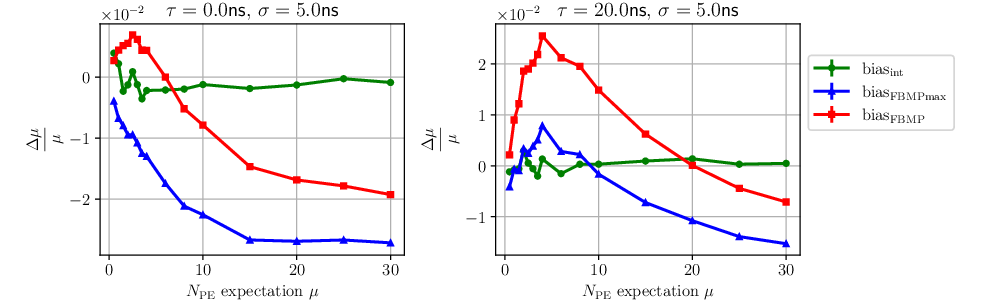
\includegraphics[width=\textwidth]{vs-biasmu-truprior.png}
\end{figure}

\section{P-FBMP using different bin width}

\begin{lstlisting}
mu_t = abs(wave.sum() / gmu)
A, wave_r, tlist, t0_t, t0_delta, cha, left_wave, right_wave = wff.initial_params(wave[::wff.nshannon], spe_pre[ent[i]['ChannelID']], Tau, Sigma, gmu, Thres['lucyddm'], p, nsp, nstd, is_t0=True, is_delta=False, n=n, nshannon=1)
mu_t = abs(wave_r.sum() / gmu)
def optit0mu(t0, mu, n, xmmse_star, psy_star, c_star, la):
    ys = np.log(psy_star) - np.log(poisson.pmf(c_star, la)).sum(axis=1)
    ys = np.exp(ys - ys.max()) / np.sum(np.exp(ys - ys.max()))
    t0list = np.arange(t0 - 3 * Sigma, t0 + 3 * Sigma + 1e-6, 0.2)
    mulist = np.arange(max(1e-8, mu - 3 * np.sqrt(mu)), mu + 3 * np.sqrt(mu), 0.1)
    b_mu = [max(1e-8, mu - 5 * np.sqrt(mu)), mu + 5 * np.sqrt(mu)]
    tlist_pan = np.sort(np.unique(np.hstack(np.arange(0, window)[:, None] + np.arange(0, 1, 1 / n))))
    As = np.zeros((len(xmmse_star), len(tlist_pan)))
    As[:, np.isin(tlist_pan, tlist)] = c_star
    assert sum(np.sum(As, axis=0) > 0) > 0

    def likelihood(x):
        a = x[0] * wff.convolve_exp_norm(tlist_pan - x[1], Tau, Sigma) / n + 1e-8 # use tlist_pan not tlist
        li = -special.logsumexp(np.log(poisson.pmf(As, a)).sum(axis=1), b=ys)
        return li

    likemu = np.array([likelihood([mulist[j], t0]) for j in range(len(mulist))])
    liket0 = np.array([likelihood([mu, t0list[j]]) for j in range(len(t0list))])
    mu, t0 = opti.fmin_l_bfgs_b(likelihood, x0=[mulist[likemu.argmin()], t0list[liket0.argmin()]], approx_grad=True, bounds=[b_mu, b_t0], maxfun=50000)[0]
    return mu, t0

truth = pelist[pelist['TriggerNo'] == ent[i]['TriggerNo']]

factor = np.sqrt(np.diag(np.matmul(A.T, A)))
A = np.matmul(A, np.diag(1. / np.sqrt(np.diag(np.matmul(A.T, A)))))
la = mu_t * wff.convolve_exp_norm(tlist - t0_t, Tau, Sigma) / n + 1e-8
xmmse, xmmse_star, psy_star, nu_star, nu_star_bk, T_star, d_tot_i, d_max_i, num_i = wff.fbmpr_fxn_reduced(wave_r, A, la, spe_pre[cid]['std'] ** 2, (gsigma * factor / gmu) ** 2, factor, len(la), stop=5, truth=truth, i=i, left=left_wave, right=right_wave, tlist=tlist, gmu=gmu, para=p)
time_fbmp = time_fbmp + time.time() - time_fbmp_start
c_star = np.zeros_like(xmmse_star).astype(int)
for k in range(len(T_star)):
    t, c = np.unique(T_star[k][xmmse_star[k][T_star[k]] > 0], return_counts=True)
    c_star[k, t] = c
maxindex = 0

xmmse_most = xmmse_star[maxindex]
pet = np.repeat(tlist[xmmse_most > 0], c_star[maxindex][xmmse_most > 0])
cha = np.repeat(xmmse_most[xmmse_most > 0] / factor[xmmse_most > 0] / c_star[maxindex][xmmse_most > 0], c_star[maxindex][xmmse_most > 0])

mu, t0 = optit0mu(t0_t, mu_t, n, xmmse_star, psy_star, c_star, la)
mu_i, t0_i = optit0mu(t0_t, mu_t, n, xmmse_most[None, :], np.array([1]), c_star[maxindex][None, :], la)
\end{lstlisting}

Motivation: to demonstrate the bin width's influence on $\mu$ bias. 

Progress: $1/n$ is the bin width, $n=\{1,2,5\}$

\begin{figure}[H]
    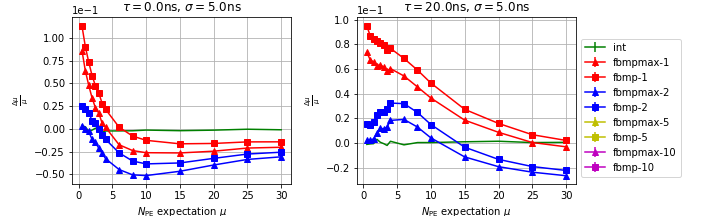
\includegraphics[width=\textwidth]{vs-biasmu-bin.png}
\end{figure}

\section{$N_{PE}$ estimation in one bin}

\begin{lstlisting}
def getm(i, p):
    N = 10000
    bias = np.empty(N)
    np.random.seed(i)
    Mu = 10
    gmu = 160
    gsigma = 40
    npan = np.arange(1, 50)
    for i in range(N):
        n = poisson.ppf(1 - uniform.rvs(scale=1-poisson.cdf(0, Mu), size=1), Mu).astype(int)
        cha = norm.ppf(1 - uniform.rvs(scale=1-norm.cdf(0, loc=gmu, scale=gsigma), size=n), loc=gmu, scale=gsigma)
        cha = cha.sum()
        if p:
            weight = poisson.pmf(npan, Mu) * norm.pdf(cha, loc=gmu * npan, scale=gsigma * np.sqrt(npan))
        else:
            weight = norm.pdf(cha, loc=gmu * npan, scale=gsigma * np.sqrt(npan))
        weight = weight / weight.sum()
        bias[i] = np.sum(npan * weight) - n
    m = bias.mean()
    return m
slices = np.arange(1000).T.tolist()
with Pool(100) as pool:
    resultpoisson = np.hstack([pool.starmap(getm, zip(slices, [True] * len(slices)))])
with Pool(100) as pool:
    resultflat = np.hstack([pool.starmap(getm, zip(slices, [False] * len(slices)))])
\end{lstlisting}

Motivation: to estimate bias of $\mu$ based on toy simulation in one bin

Progress: set $\mu$. Sampling: $n\sim\mathrm{Poisson}(n|\mu)$, $q_i\sim\mathrm{Gaussian}(q_i|1,\sigma_q^2),i=\{1,\cdots,n\}$, $Q=\sum_i q_i$. Estimation: $p(n|Q) = \frac{\mathrm{Poisson}(n|\mu) \cdot \mathrm{Gaussian}(Q|n,n\sigma_q^2)}{\sum_{j=1}^n \mathrm{Poisson}(j|\mu) \cdot \mathrm{Gaussian}(Q|j,j\sigma_q^2)}$ or $p(n|Q) = \frac{\mathrm{Gaussian}(Q|n,n\sigma_q^2)}{\sum_{j=1}^n \mathrm{Gaussian}(Q|j,j\sigma_q^2)}$

Result: when using Poisson prior, there is \textbf{no} bias, when using flat prior, there is bias. 

\begin{figure}[H]
    \centering
    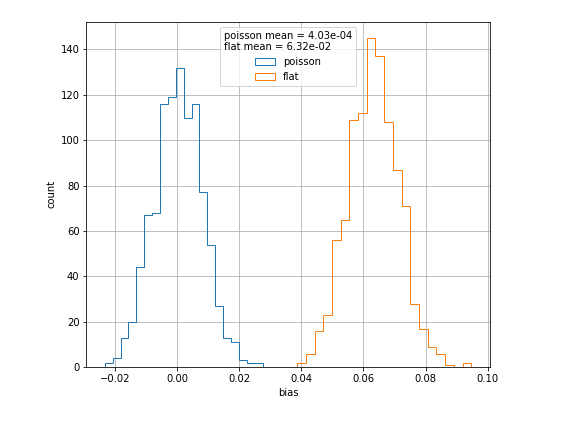
\includegraphics[width=0.5\textwidth]{onebinbias.png}
\end{figure}

\section{$N_{PE}$ estimation based on toy simulation}

\begin{lstlisting}
n = 10000
npe = 30
noi = True
if noi:
    std = 1.
else:
    std = 1e-4
window = 200
np.random.seed(0)
wdtp = np.dtype([('No', np.uint32), ('Waveform', np.float, window)])
waves = np.empty(n).astype(wdtp)
tlist = np.repeat(np.array([0, 1, 1]), npe / 3)
sams = [np.vstack((tlist, wff.charge(npe, gmu=gmu, gsigma=gsigma, thres=0))).T for i in range(n)]
pan = np.arange(0, window)
t0 = 0.5
for i in tqdm(range(n)):
    wave = np.sum([np.where(pan > sams[i][j, 0], wff.spe(pan - sams[i][j, 0], tau=p[0], sigma=p[1], A=p[2]) * sams[i][j, 1] / gmu, 0) for j in range(len(sams[i]))], axis=0)
    if noi:
        wave = wave + np.random.normal(0, std, size=window)
    waves[i]['Waveform'] = wave
waves['No'] = np.arange(n).astype(np.uint32)
sdtp = np.dtype([('No', np.uint32), ('HitPosInWindow', np.float64), ('Charge', np.float64)])
pelist = np.empty(sum([len(sams[i]) for i in range(n)])).astype(sdtp)
pelist['No'] = np.repeat(np.arange(n), [len(sams[i]) for i in range(n)]).astype(np.uint32)
pelist['HitPosInWindow'] = np.hstack([sams[i][:, 0] for i in range(n)])
pelist['Charge'] = np.hstack([sams[i][:, 1] for i in range(n)])
mu = np.empty(n)
for i in tqdm(range(n)):
    wave = waves[i]['Waveform'].astype(np.float64) * spe_pre[0]['epulse']
    truth = pelist[pelist['No'] == waves[i]['No']]
    tlist = np.unique(truth['HitPosInWindow'])

    t_auto = np.arange(0, window)[:, None] - tlist
    A = p[2] * np.exp(-1 / 2 * (np.log((t_auto + np.abs(t_auto)) / p[0] / 2) / p[1]) ** 2)
    mu_t = npe
    factor = np.sqrt(np.diag(np.matmul(A.T, A)))
    A = np.matmul(A, np.diag(1. / np.sqrt(np.diag(np.matmul(A.T, A)))))
    la = mu_t * np.array([1, 2]) / 3
    
    xmmse, xmmse_star, psy_star, nu_star, nu_star_bk, T_star, d_tot_i, d_max_i, num_i = wff.fbmpr_fxn_reduced(wave, A, la, std ** 2, (gsigma * factor / gmu) ** 2, factor, len(la), stop=5)
    
    c_star = np.zeros_like(xmmse_star).astype(int)
    for k in range(len(T_star)):
        t, c = np.unique(T_star[k][xmmse_star[k][T_star[k]] > 0], return_counts=True)
        c_star[k, t] = c

    mu[i] = np.average(c_star.sum(axis=1), weights=psy_star)
\end{lstlisting}

Motivation: try to understand the relation between convolution process and bias

Progress: there is no $\mu$, set $N_{PE}$ as 30, set \textit{HitPosInWindow} to $[0, 1]$, set time profile prior as $[1/3, 2/3]$, sample \textit{Charge}. Use FBMP to generate posterior distribution of $N_{PE}$. 

Result: there is \textbf{no} bias on this configuration

\begin{figure}[H]
    \centering
    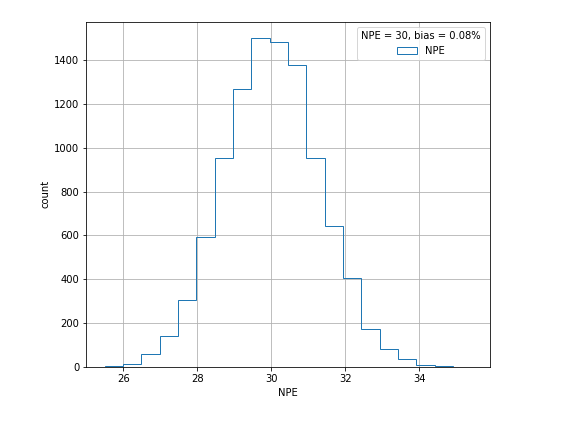
\includegraphics[width=0.5\textwidth]{toybias.png}
\end{figure}

\section{Influence of lucyddm \texttt{tlist} initialization on $\mu$ bias}

\begin{lstlisting}
n = 2
A, wave_r, tlist, t0_t, t0_delta, cha, left_wave, right_wave = wff.initial_params(wave[::wff.nshannon], spe_pre[ent[i]['ChannelID']], Tau, Sigma, gmu, Thres['lucyddm'], p, nsp, nstd, is_t0=True, is_delta=False, n=n, nshannon=1)

truth = pelist[pelist['TriggerNo'] == ent[i]['TriggerNo']]

c_star_truth = np.sum([np.where(tlist - 0.5 / n < truth['HitPosInWindow'][j], 1, 0) * np.where(tlist + 0.5 / n > truth['HitPosInWindow'][j], 1, 0) for j in range(len(truth))], axis=0)

mu = c_star_truth.sum()
t0 = t0_t
\end{lstlisting}

Motivation: to test the influence of lucyddm time bin initialization on $\mu$ bias

Progress: lucyddm initialization, estimate $\mu$ as number of truth \textit{HitPosInWindow} in \texttt{tlist}

Result: there is \textbf{no} bias from lucyddm \texttt{tlist} initialization

\begin{figure}[H]
    \centering
    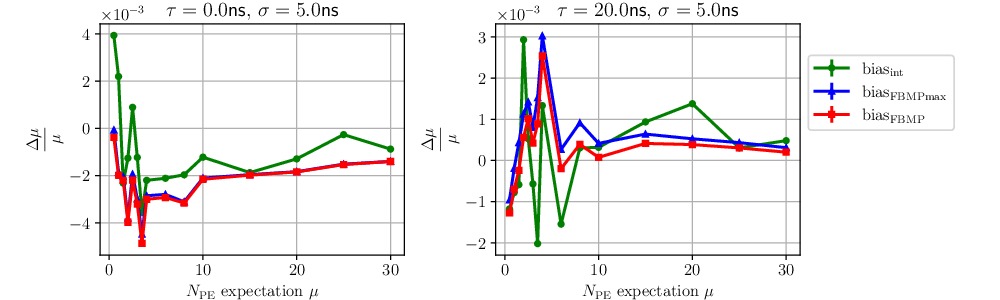
\includegraphics[width=\textwidth]{vs-biasmu-lucyddmtlist.png}
\end{figure}

\section{Influence of lucyddm \texttt{wave\_r} initialization on $\mu$ bias}

\begin{lstlisting}
mu_t = abs(wave.sum() / gmu)
n = 2
A, wave_r, tlist, t0_t, t0_delta, cha, left_wave, right_wave = wff.initial_params(wave[::wff.nshannon], spe_pre[ent[i]['ChannelID']], Tau, Sigma, gmu, Thres['lucyddm'], p, nsp, nstd, is_t0=True, is_delta=False, n=n, nshannon=1)
mu_t = abs(wave_r.sum() / gmu)
mu = mu_t
t0 = t0_t
\end{lstlisting}

Motivation: to test the influence of waveform cut in lucyddm initialization on $\mu$ bias

Progress: lucyddm initialization, estimate $\mu$ as number of integral of truncated waveform \texttt{wave\_r}

Result: there is \textbf{no} bias from lucyddm waveform cut initialization

\begin{figure}[H]
    \centering
    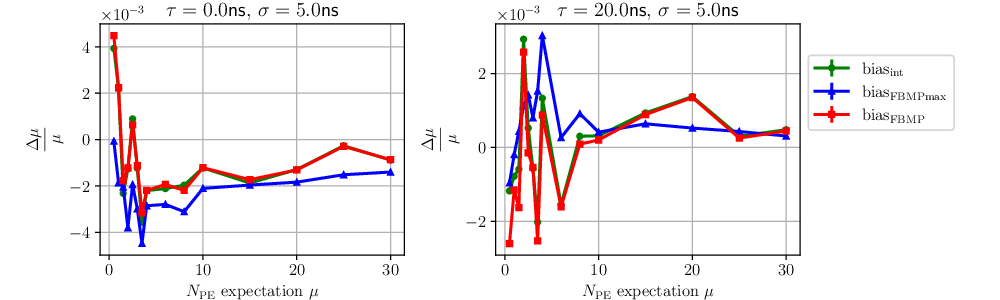
\includegraphics[width=\textwidth]{vs-biasmu-lucyddmwave.png}
\end{figure}

\end{document}